\chapter{\IfLanguageName{dutch}{Proof of concept}{State of the art}}%
\label{ch:proof-of-concept}

Dit deel van het onderzoek stelt een Proof of Concept voor die zich richt op het web scrapen van het netwerkverkeer van een website zodat de gestructureerde data die verstuurd wordt van de server kan onderschept worden. Sommige van deze bestanden die de server verstuurt, bevatten de gestructureerde data die de website gebruikt om zijn inhoud dynamisch te genereren. In deze gestructureerde data is vaak meer informatie te vinden dan op de website getoond wordt. Dit zorgt voor een verhoogde kwaliteit van verzamelde data. Het vergt ook minder verwerkingscapaciteit van de machine waarop de scraper uitgevoerd wordt omdat de HTML-code niet geparsed hoeft te worden. De Proof of Concept bestaat uit een Python script.

\section{Vereisten}
Het uitvoeren van deze Proof of Concept vereist bepaalde software op het systeem. De vereiste software zijn:
\begin{itemize}
    \item Python \footnote{\url{https://www.python.org/downloads/}}
    \item De package manager pip~\footnote{\url{https://pip.pypa.io/en/stable/installation/}}
\end{itemize}

\section{Versies}
In deze Proof of Concept wordt gebruik gemaakt van Python versie 3.10.2. De python-Bibliotheken die in deze Proof of Concept gebruikt zullen worden zijn:

\begin{itemize}
    \item \textbf{json: } Deze Python-bibliotheek wordt gebruikt om met JSON-bestanden te werken. json is standaard geinstalleerd in Python

    \item \textbf{Requests: } Deze Python-bibliotheek wordt gebruikt om HTTP-verzoeken te maken.

    \item \textbf{Selenium: } Selenium wordt gebruikt om het netwerkverkeer op te halen.
\end{itemize}

Om mogelijke conflicten tussen de gebruikte Python-bibliotheken te voorkomen wordt gebruik gemaakt van een virtuele Python omgeving. Om de virtuele omgeving te creëren moet het commando \ref{cmd:createvenv} uitgevoerd worden.

\begin{lstlisting}[language=bash, label={cmd:createvenv}, caption={Het commando om een virtuele Python omgeving te creëren}]
    python -m venv /path/to/new/virtual/environment/
\end{lstlisting}
Om de virtuele Python omgeving te activeren op een Windows machine moet het commando \ref{cmd:startvenv} uitgevoerd worden, voor een Linux of MacOS machine moet het commando \ref{bash:startvenv} gebruikt worden.
\begin{lstlisting}[language=bash, label={cmd:startvenv}, caption={Het commando om een virtuele Python omgeving te activeren op een Windows machine}]
    venv\Scripts\activate.bat
\end{lstlisting}

\begin{lstlisting}[language=bash, label={bash:startvenv}, caption={Het commando om een virtuele Python omgeving te activeren op een Linux of MacOS machine}]
    $ source myvenv/bin/activate
\end{lstlisting}

Om de gebruikte Python-bibliotheken te installeren moet het commando \ref{cmd:req.txt} uitgevoerd worden. het bestand \texttt{requirements.txt} is te vinden op de github-pagina \footnote{\url{https://github.com/hannesroegiers/bachelorproef/tree/main/PoC}}van deze Proof of Concept. Dit bestand bevat de nodige Python-bibliotheken met de gebruikte versie.
\begin{lstlisting}[language=bash, label={cmd:req.txt}, caption={Het commando om de nodige Python-bibliotheken te installeren}]
    pip install -r requirements.txt
\end{lstlisting}

\section{Verkenning}
Op de doel website\footnote{\url{https://www.oddsportal.com/football/belgium/jupiler-pro-league/}} zijn een aantal voetbal wedstrijden te zien. Naast iedere wedstrijd staan 3 kolommen zoals te zien in \ref{fig:website1}. De cijfers(betting odds voor de wedstrijden) die in deze kolommen staan zijn de data die de scraper gaat proberen te extraheren.

\begin{figure}[h]
    \centering
    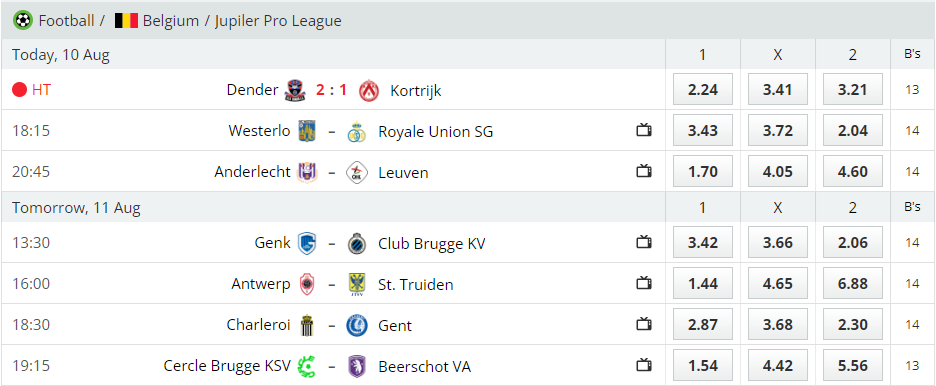
\includegraphics[width=\linewidth]{graphics/website1.png}
    \caption{De doel website}
    \label{fig:website1}
\end{figure}

\section{Manuele analyse}
\label{sec:analyse}
In deze tweede fase van het onderzoek wordt gebruik gemaakt van de Chrome-browser en de ingebouwde developer tools om het netwerkverkeer van een website te analyseren. De developer tools kunnen worden geopend door op de functietoets \texttt{F12} te drukken of door met de rechtermuisknop op een webpagina te klikken en vervolgens te kiezen voor \texttt{Inspect} of \texttt{Inspecteren}.
\\
Bij het laden van een website worden verschillende HTTP-verzoeken naar de server gestuurd, waarvan de antwoorden dienen om de inhoud van de website dynamisch op te bouwen. Deze HTTP-verzoeken en hun antwoorden zijn te vinden in het \texttt{Network}-tabblad van de developer tools, waar het netwerkverkeer van de website in detail wordt weergegeven.

Voor web scraping zijn twee specifieke tabbladen in de developer tools van belang: het \texttt{Elements}-tabblad en het \texttt{Network}-tabblad. In het \texttt{Elements}-tabblad kan de HTML-code en structuur van de website worden bekeken. Dit biedt inzicht in hoe de inhoud van de website is opgebouwd. In het \texttt{Network}-tabblad kan het netwerkverkeer tussen de client(de browser) en de server worden geanalyseerd, zoals geïllustreerd in figuur~\ref{fig:networktab}.

\begin{figure}[h]
    \centering
    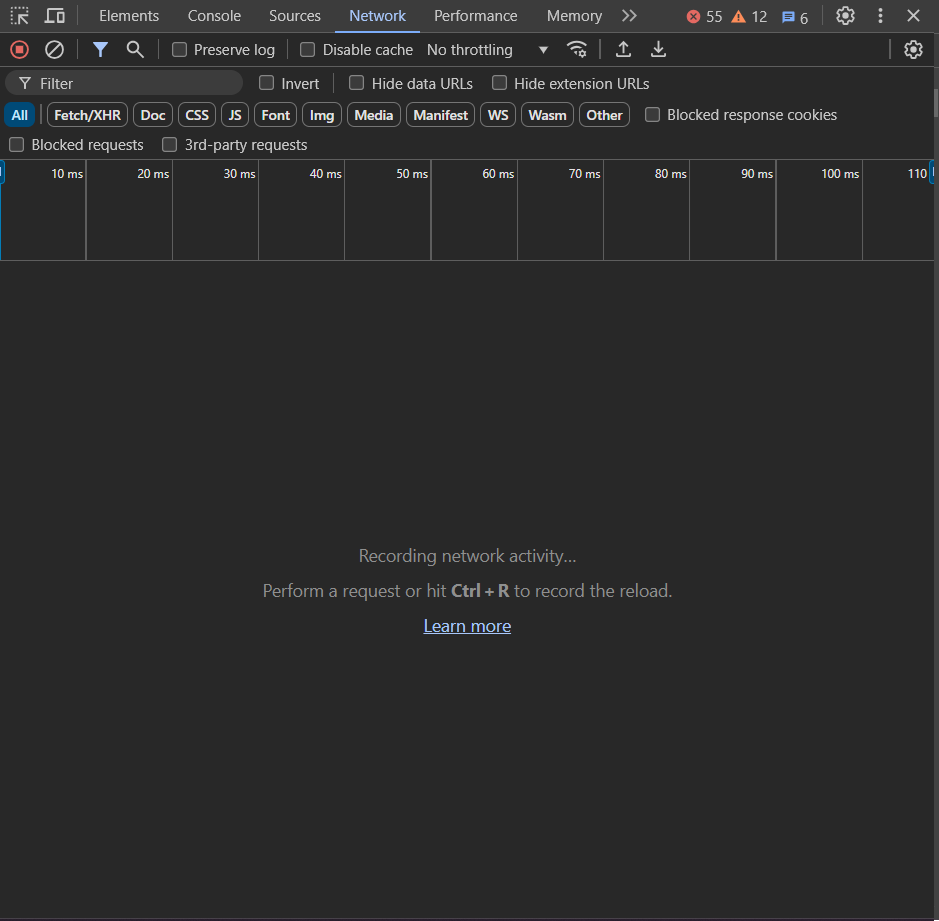
\includegraphics[width=\linewidth]{graphics/DevTools1.png}
    \caption{De developer tools, het netwerk tabblad}
    \label{fig:networktab}
\end{figure}

Wanneer de webpagina opnieuw wordt geladen, worden in het Network-tabblad alle netwerkverzoeken weergegeven die plaatsvinden tussen de client en de server, zoals te zien is in figuur~\ref{fig:networktab2}.

\begin{figure}[h]
    \centering
    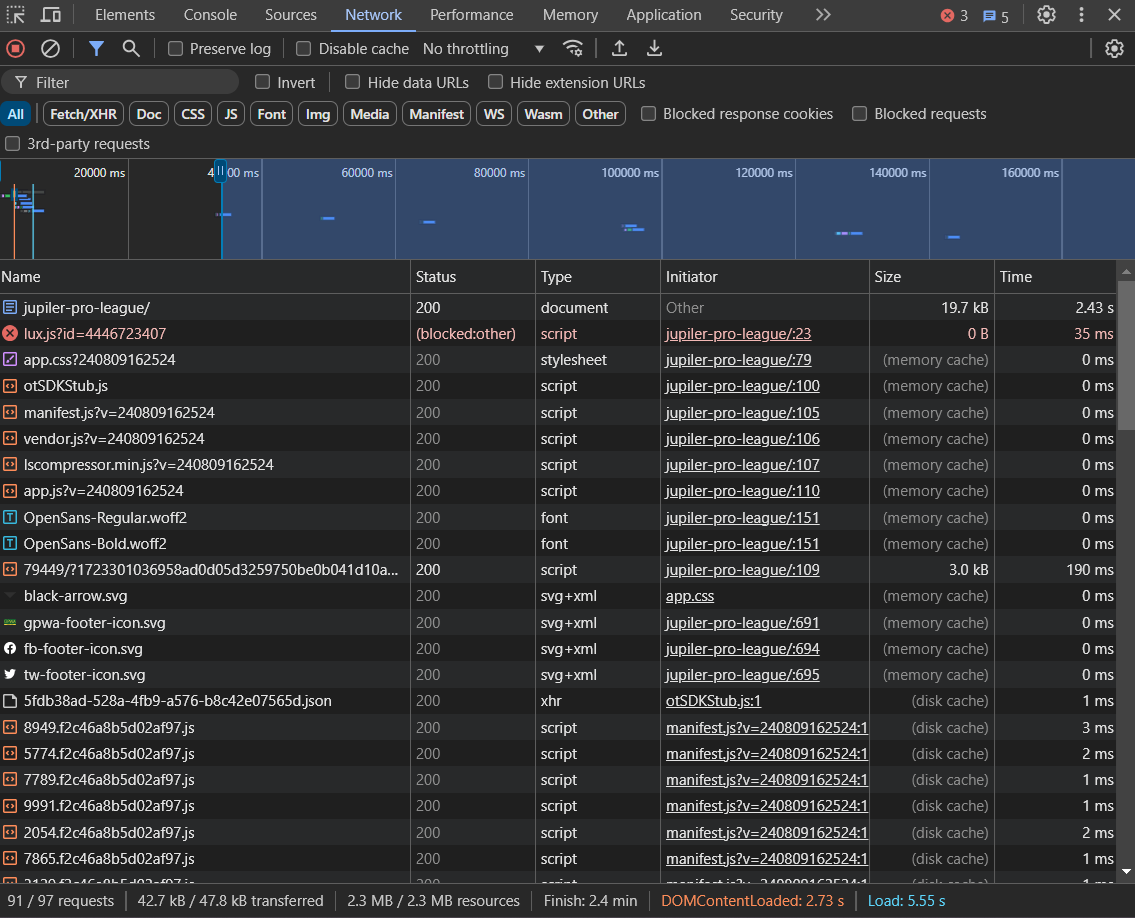
\includegraphics[width=\linewidth]{graphics/DevTools2.png}
    \caption{Het netwerkverkeer in de developer tools}
    \label{fig:networktab2}
\end{figure}

Hoewel er veel verschillende soorten bestanden worden uitgewisseld, richt dit onderzoek zich op bestanden die gestructureerde data bevatten. In de developer tools kan dit verkeer manueel worden gefilterd door de optie \texttt{Fetch/XHR} te selecteren. Deze filter toont voornamelijk JSON- en XML-bestanden, die vaak belangrijke data bevatten voor verdere analyse.
Er blijven nu slechts 7 requests over zoals te zien in figuur~\ref{fig:networktab3}.

\begin{figure}[h]
    \centering
    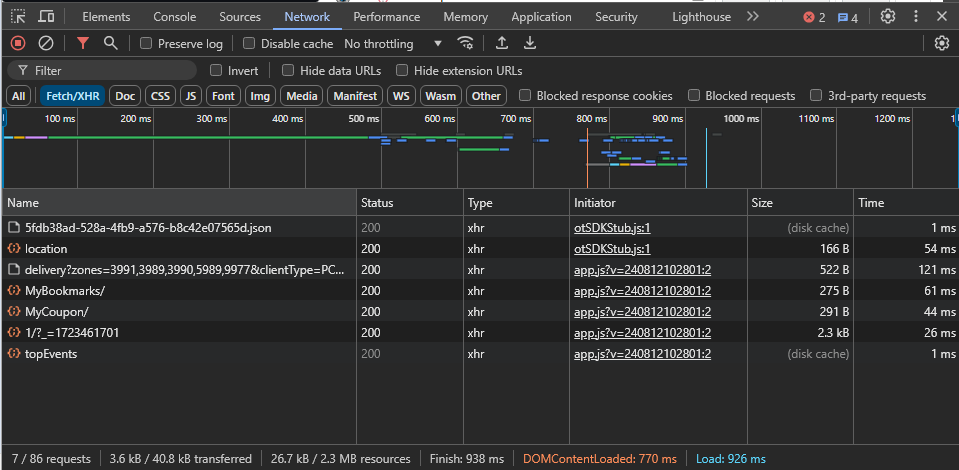
\includegraphics[width=\linewidth]{graphics/DevTools3.png}
    \caption{Het gefilterde netwerkverkeer in de developer tools}
    \label{fig:networktab3}
\end{figure}

De antwoorden van deze overblijvende HTTP-verzoeken bevatten allemaal JSON-bestanden. Na verdere manuele analyse van deze bestanden is vast te stellen dat de betting odds terug te vinden zijn in het HTTP-verzoek dat een bestand met naam \texttt{?\_=1723461701} terug geeft.

\subsubsection{Bepalen van de web scraping methode}
De HTML-code van de doel website is complex, hierdoor is de code moeilijk te lezen en kleine veranderingen in de code kunnen ervoor zorgen dat de locatie van de betting odds verandert. De website wordt dynamisch opgebouwd met behulp van HTTP-verzoeken die gestructureerde data opvragen. Dit zorgt ervoor dat web scraping met netwerkverkeersanalyse bij deze website de beste keuze is.
\\
\\
In figuur~\ref{fig:networktab4} is te zien hoe de header van het HTTP-verzoek is opgebouwd. Indien de website een duidelijke en consistente structuur in de headers heeft, kan een Python-script worden ontwikkeld dat gebruik maakt van een lus om systematisch HTTP-requests te versturen. Deze aanpak maakt het mogelijk om alle benodigde data te verzamelen zonder de beperkingen van traditionele scraping-methoden die zich puur op de HTML-content richten.
\begin{figure}[h]
    \centering
    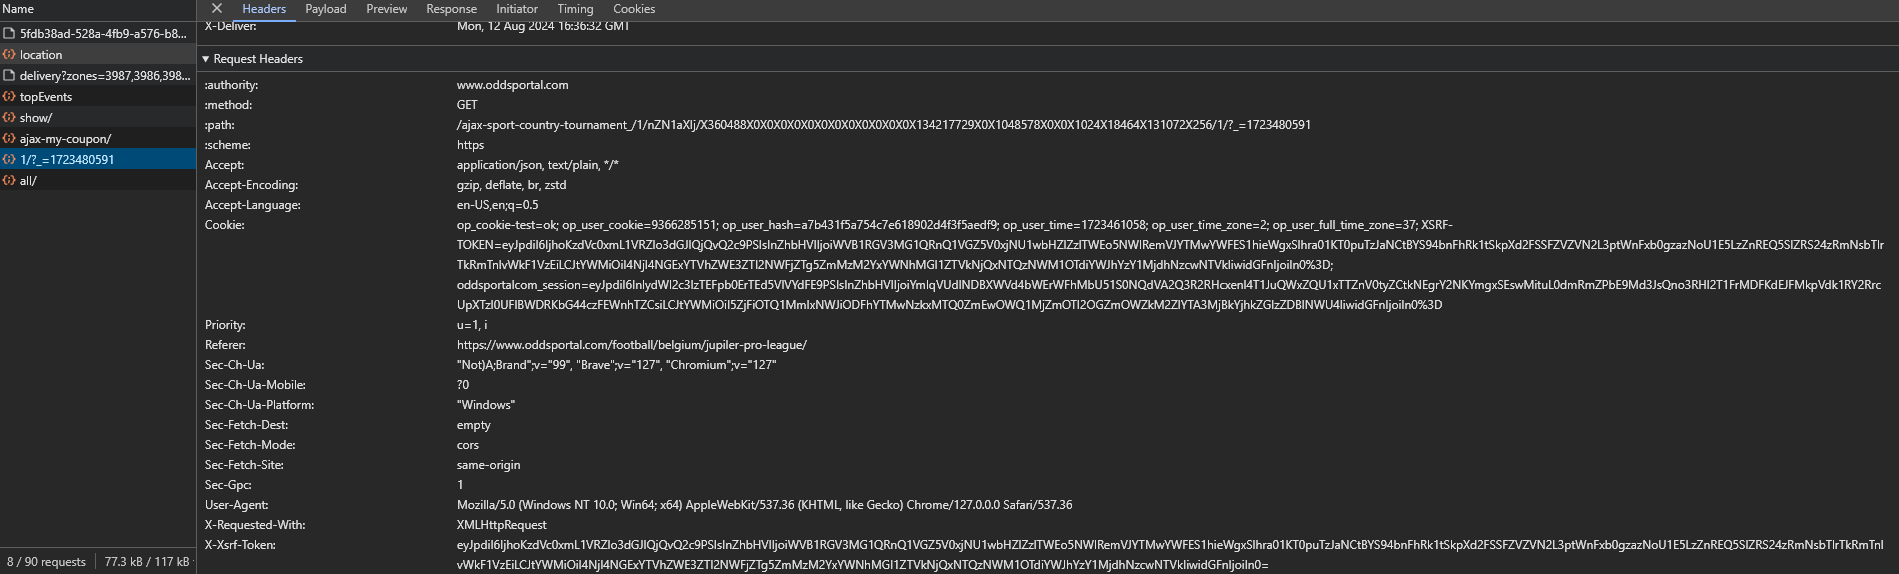
\includegraphics[width=\linewidth]{graphics/headers.png}
    \caption{De headers van het betting odds HTTP-verzoek}
    \label{fig:networktab4}
\end{figure}


De Python-loop stuurt hierbij een reeks gestructureerde HTTP-verzoeken naar de server van de doelwebsite. Door gebruik te maken van variabelen in de URL of parameters binnen de request headers, kan het script automatisch door verschillende datasets navigeren en deze extraheren. Dit minimaliseert de kans op blokkades door anti-scraping maatregelen en verhoogt de efficiëntie van de data-extractie. In code fragment~\ref{code:example5} is een voorbeeld te zien over web scrapen met netwerkverkeersanalyse wanneer de parameters in de HTTP-verzoek header gestructureerd en niet vertroebeld zijn.
\begin{listing}
    \begin{lstlisting}[language=python, captionpos=b, caption={Een voorbeeld van een eenvoudige webscraper.}, label={code:example5}]
        import requests

        # Dummy URL: https://www.oddsportal.com/ajax-sport-country-tournament/sport/country/league/

        # Deze arrays kunnen manueel onderhouden worden of opgehaald worden met een API
        request_parameters = {
            "Voetbal": {
                "Belgie": ["Jupiler Pro League", "Eerste klasse B"],
                "Nederland": ["Eredivisie", "Eerste Divisie"],
                "Engeland": ["Premier League", "Championship"],
            },
            "Hockey": {
                "België": ["Belfius Hockey League"],
                "Nederland": ["Hoofdklasse", "Promotieklasse"],
                "Duitsland": ["Bundesliga"],
            },
            "Tennis": {
                "Internationaal": ["ATP Tour", "WTA Tour"],
                "Verenigde Staten": ["US Open Series"],
                "Australie": ["Australian Open"],
            }
        }

        # Overlopen van alle url parameters
        for sport, countries in request_parameters.items():
            for country, leagues in countries.items():
                for league in leagues:
                    request_string = f"https://www.oddsportal.com/ajax-sport-country-tournament/{sport}/{country}/{league}/"
                    r = requests.get(request_string)
    \end{lstlisting}
\end{listing}

Na een grondige analyse van het HTTP-verzoek kan echter worden geconcludeerd dat er in dit geval geen duidelijke en consistente structuur aanwezig is in het verzoek. De parameters die in het verzoek worden gebruikt, lijken opzettelijk vertroebeld (geobfusceerd) te zijn, waardoor ze bestaan uit willekeurige tekens zonder directe betekenis. Dit maakt het onmogelijk om de inhoud en betekenis van deze parameters zonder meer te interpreteren. Om enige nuttige informatie hieruit te kunnen destilleren, zou het noodzakelijk zijn om de bijbehorende JavaScript-code te reverse-engineeren. Dit proces zou echter aanzienlijke tijd en diepgaande technische kennis vereisen.
\\ \\
Een van de parameters in het verzoek komt overeen met het bestand dat als antwoord wordt teruggestuurd. Hoewel de inhoud van dit bestand constant blijft bij het herladen van de pagina, verandert de naam van het bestand bij elke herlaadbeurt, het enige dat consistent blijft bij deze naam is dat het start met \texttt{?\_=17}. Deze naamwijziging voegt een extra laag van complexiteit toe, waardoor verdere analyse van deze parameter bijzonder uitdagend is.
\\ \\
De web scraping methode die daarom zal worden toegepast voor deze website maakt gebruik van netwerkverkeersanalyse. Het volledige netwerkverkeer zal worden opgehaald en dan daarna gefilterd worden op bestandstype, naam en inhoud. De focus zal liggen op robuustheid en minimaal onderhoud.

\section{Ontwikkeling van Proof of Concept}
De volgende afbeelding~\ref{fig:flowchart2} geeft de flow van de web scraper weer.
\begin{figure}[h]
    \centering
    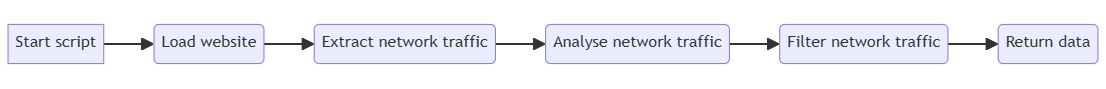
\includegraphics[width=\linewidth]{graphics/flow-chart2.png}
    \caption{Het gefilterde netwerkverkeer in de developer tools}
    \label{fig:flowchart2}
\end{figure}

De web scraper maakt gebruik van volgende Python-bibliotheken~\ref{code:poc1}.
\\ \\
Selenium wordt gebruikt om de pagina te laden en \texttt{Options} zijn nodig zodat kan worden meegegeven aan de web scraper dat het netwerkverkeer van de browser moet worden onthouden. De Python-bibliotheek json wordt gebruikt om met JSON-bestanden te werken en de requests bibliotheek wordt gebruikt om HTTP-verzoeken te sturen.

\begin{lstlisting}[language=python, captionpos=b, caption={De imports voor Proof of Concept.}, label={code:poc1}]
    from selenium.webdriver.chrome.options import Options
    from selenium import webdriver
    import json
    import requests
\end{lstlisting}

\subsection{Ophalen en filteren van netwerkverkeer}
Het eerste deel van de Proof of Concept focust zich op het ophalen en filteren van het netwerkverkeer dat loopt tussen de website en de server. De lijst met HTTP-verzoeken die op het einde van deze stap overblijft, zijn de HTTP-verzoeken die deze website gebruikt om zijn inhoud dynamisch op te bouwen.
\\ \\
In deze stap wordt een instantie van de \texttt{Options}-klasse aangemaakt en wordt de mogelijkheid geconfigureerd om de performance logs te verkrijgen. Hierna wordt de Chrome-webdriver geïnitialiseerd  met de eerde ingestelde opties. Dit stelt de scraper in staat om netwerkverkeer te monitoren tijdens het laden van de webpagina.
\begin{lstlisting}[language=python, captionpos=b, caption={De imports voor Proof of Concept.}, label={code:poc2}]
    options = Options()
    options.set_capability('goog:loggingPrefs', {'performance': 'ALL'})
    driver = webdriver.Chrome(options=options)
\end{lstlisting}

In code-fragment~\ref{code:poc3} wordt de webdriver naar de opgegeven URL gestuurd. In dit geval is de URL een pagina van de Jupiler Pro League op OddsPortal. Het laden van de pagina genereert netwerkverkeer dat kan worden geanalyseerd en opgeslagen in de variabele \texttt{logs}. Tot slot wordt de webdriver afgesloten om alle resources vrij te geven.

\begin{lstlisting}[language=python, captionpos=b, caption={Ophalen van het netwerkverkeer}, label={code:poc3}]
    url = "https://www.oddsportal.com/football/belgium/jupiler-pro-league/"
    driver.get(url)
    performance_logs = driver.get_log("performance")
    driver.quit()
\end{lstlisting}

Bij code-fragment~\ref{code:poc4} worden de \texttt{performance-logs} gefilterd zodat enkel nog de HTTP-verzoeken en -antwoorden overblijven. Aangezien iedere item in \texttt{performance-log}wordt opgeslagen als een JSON-object, wordt elke entry afzonderlijk ingeladen en verwerkt als een JSON-bestand. Dit stelt ons in staat om specifieke eigenschappen van de HTTP-verzoeken en -antwoorden te extraheren, zoals headers en parameter type.

\begin{lstlisting}[language=python, captionpos=b, caption={Filteren van performance-logs }, label={code:poc4}]
    filtered_logs = []
    filter_list = ["Network.request", "Network.response"]

    for entry in performance_logs:
        networktraffic = json.loads(entry["message"])["message"]
        if any(keyword in networktraffic["method"] for keyword in filter_list):
            filtered_logs.append(networktraffic)
\end{lstlisting}

In onderstaande code-fragment~\ref{code:poc5}  worden de \texttt{filtered\_logs} doorlopen om alleen de URL's van de HTTP-verzoeken met type XHR te verzamelen in een lijst. Door te filteren op XHR-verzoeken richt de code zich uitsluitend op die verzoeken waarin doorgaans gestructureerde data zoals JSON wordt verzonden.

\begin{lstlisting}[language=python, captionpos=b, caption={De URL's uit de HTTP-verzoeken halen}, label={code:poc5},]
    urls = []
    for log in filtered_logs:
        try:
            if(log["params"]["type"] == 'XHR'):
                url = log["params"]["request"]["url"]
                urls.append(url)
        except:
            pass
\end{lstlisting}


In code-fragment~\ref{code:poc6} worden de verzamelde URL's verder gefilterd om specifieke bestandstypen en paden uit te sluiten die niet relevant zijn voor de analyse. Dit omvat onder andere afbeeldingen, JavaScript-bestanden, CSS-bestanden en icon-bestanden. De lijst \texttt{filtered\_urls} HTTP-verzoeken die gestructureerde data terug geven.
\begin{lstlisting}[language=python, captionpos=b, caption={Ongewenste bestanden filteren}, label={code:poc6}]
    filter_list = [".svg", ".png", "/js/", ".js", ".css", ".ico"]
    filtered_urls = [url for url in urls if not any(filter_str in url for filter_str in filter_list)]
\end{lstlisting}

Het resultaat van het eerste deel van de Proof of Concept is een verzameling van HTTP-verzoeken die gestructureerde data teruggeven. Deze data wordt door de website gebruikt om de inhoud dynamisch op te bouwen.

\subsection{Filteren op basis van inhoud}
In het tweede deel van de Proof of Concept worden de overgebleven HTTP-verzoeken gefilterd en gerangschikt op basis van inhoud. Er zijn meerdere manieren om deze data te filteren zoals reguliere expressies of full-text search. De gekozen methode hangt af van de data waar men naar op zoek is. In dit geval is het voldoende om op de aanwezigheid van bepaalde woorden te controleren. Omdat de data waar we naar opzoek zijn numeriek is, is er dus geen nood aan reguliere expressies of full-text search.
\\ \\
In het eerste codefragment van dit gedeelte, weergegeven in code~\ref{code:poc7}, wordt een functie gedefinieerd die een HTTP-verzoek verstuurt naar de opgegeven URL. Wanneer dit verzoek succesvol is, wordt de inhoud van het HTTP-antwoord verder geanalyseerd. De manier waarop deze inhoud wordt geanalyseerd, is afhankelijk van zowel het type data waarnaar gezocht wordt als de manier waarop de server deze data retourneert. In deze Proof of Concept wordt specifiek gezocht naar numerieke data. Daarom is het voldoende om te zoeken naar bepaalde trefwoorden die de variabelen van de gezochte numerieke data representeren.

\begin{lstlisting}[language=python, captionpos=b, caption={Filteren van performance-logs }, label={code:poc7}]
    import re

    def check_url_contents(url, words=None, regex_patterns: list=None):
        headers = {
            "User-Agent": "Mozilla/5.0 (Windows NT 10.0; Win64; x64) AppleWebKit/537.36 (KHTML, like Gecko) Chrome/58.0.3029.110 Safari/537.3"
        }
        response = requests.get(url, headers=headers)

        results = {'words': {}, 'regex_patterns': {}}

        if response.status_code == 200:
            content = response.text

            if words:
                for word in words:
                    count = content.lower().count(word.lower())
                    results['words'][word] = count

                if regex_patterns:
                    for regex in regex_patterns:
                        pattern = re.compile(regex)
                        matches = pattern.findall(content)
                        results['regex_patterns'][regex] = len(matches)

        return results
\end{lstlisting}

In aanvulling op de eerder genoemde functie is er ook een functie genaamd \texttt{rank\_urls} geïmplementeerd. Deze functie sorteert de URL's op basis van de frequentie waarmee specifieke woorden of reguliere expressies voorkomen in de bijbehorende bestanden. Dit is vooral nuttig in situaties waarin er meerdere URL's overblijven en het niet mogelijk is om met absolute zekerheid te bepalen welk bestand de juiste data bevat, zonder elk bestand handmatig te openen en te controleren. Het willekeurig verwijderen van bestanden is in dit geval geen optie, omdat we niet volledig zeker kunnen zijn welk bestand de correcte gegevens bevat. Door de URL's te rangschikken op basis van de overeenkomst met de verwachte inhoud, wordt het eenvoudiger om de meest relevante bestanden te identificeren.
\\ \\
In het laatste codefragment~\ref{code:poc8} worden de gerangschikte URL's weergegeven. Het gebruik van de regel \lstinline|if entry[1] < 1| zorgt ervoor dat de lus stopt zodra een URL wordt gevonden die niet aan de criteria voldoet. Aangezien de URL's vooraf gerangschikt zijn op basis van relevantie, betekent dit dat alle volgende URL's ook niet aan de criteria zullen voldoen. Hierdoor wordt enkel de eerste reeks URL's die aan de voorwaarden voldoen, weergegeven.
De zoekwoorden die in code-fragment worden gebruikt, zijn gebaseerd op de manuele analyse van de website in sectie \ref{sec:analyse}.
\begin{lstlisting}[language=python, captionpos=b, caption={Filteren van performance-logs }, label={code:poc8}]
    result = rank_urls(filtered_urls, ['odd', 'bet', 'average', 'avg'])

    for index, entry in enumerate(result, start=1):
        if entry[1] < 1:
            break
    print(f"{index}: {entry[0]}")
\end{lstlisting}

De zoekwoorden die in bovenstaand code-fragment~\ref{code:poc8} worden gebruikt, zijn gebaseerd op de manuele analyse van de website in sectie \ref{sec:analyse}.

\section{resultaten}
bespreken van de resultaten. Grafiek die de duur van de scraper toont en hoelang elk deel duurde (ophalen van de requests en het verwerken ervan). Ik ga deze scraper op een aantal paginas van de website laten lopen zodat er meer tijds data is om mij op te baseren.
\\\\

Het resultaat van deze Proof of Concept is een webscraper die door middel van netwerkverkeersanalyse op zoek gaat naar de gestructureerde data die op de website beschikbaar is. Dit Python-script automatiseert het proces door de URL's in de HTTP-verzoeken te identificeren die de website gebruikt om de benodigde gegevens op te halen. Hierdoor is het niet langer nodig om het netwerkverkeer handmatig te analyseren, wat zowel tijd bespaart als de nauwkeurigheid van de gegevensverzameling verbetert.
De uitvoeringstijd van dit Python-script is nauwkeurig gemeten en opgedeeld in drie afzonderlijke fasen. In de eerste fase wordt het netwerkverkeer opgehaald, in de tweede fase wordt dit verkeer gefilterd, en in de derde fase wordt de inhoud van de gevonden URL's geanalyseerd. Tijdens fase 1 en 3 worden HTTP-verzoeken verzonden, terwijl in fase 2 de data uitsluitend lokaal wordt verwerkt.
\\ \\
De figuur~\ref{fig:time_graph} geeft de uitvoeringstijd van de web scraper weer, gemeten in seconden, er zijn op de grafiek 50 metingen te zien. Elk punt op de x-as vertegenwoordigt een enkele iteratie van de web scraper. De uitvoeringstijd is onderverdeeld in vier componenten: sectie 1 (het ophalen van het netwerkverkeer), sectie 2 (het filteren van het netwerkverkeer), sectie 3 (het analyseren van de URL-inhoud), en de totale tijd, die de som is van deze drie secties.
In de grafiek zijn vier duidelijke pieken zichtbaar, voornamelijk in secties 1 en 3. In sectie 2 ontbreken deze pieken echter, wat te verklaren is doordat sectie 2 geen HTTP-verzoeken verstuurt. Hierdoor wordt deze sectie niet beïnvloed door externe factoren zoals netwerksnelheid of serverrespons, wat in tegenstelling staat tot de secties 1 en 3.
\\ \\
De pieken in secties 1 en 3 wijzen erop dat de variatie in uitvoeringstijd grotendeels wordt bepaald door de snelheid van de server en de website waarmee de scraper communiceert. Dit wordt verder ondersteund door de standaarddeviatie in figuur~\ref{fig:time_table} De standaarddeviatie in secties 1 en 3 is namelijk aanzienlijk hoger dan die in sectie 2, wat de invloed van externe factoren op de uitvoeringstijd bevestigt.
\begin{figure}[ht]
\pgfplotstableread[col sep=comma,]{../times2.csv}\datatable
\begin{tikzpicture}
   \begin{axis}[
       width=\textwidth,
       height=10cm,
       xtick=data,
       xticklabels from table={\datatable}{x-axis},
       x tick label style={font=\normalsize, rotate=35, anchor=east},
       legend style={at={(0.98,0.3)},anchor=south east},
       ylabel={time(s)},
       xlabel={Iteraties van de web scraper}]

    \addplot[blue!80 ] table [x expr=\coordindex, y={Section 1}] {\datatable};
    \addlegendentry{Sectie 1}

    \addplot[red!80 ] table [x expr=\coordindex, y={Section 2}] {\datatable};
    \addlegendentry{Sectie 2}

    \addplot[green!80 ] table [x expr=\coordindex, y={Section 3}] {\datatable};
    \addlegendentry{Sectie 3}

    \addplot[orange!80 ] table [x expr=\coordindex, y={Total}] {\datatable};
    \addlegendentry{Totaal}

%    \addplot [dashed, thin, black] coordinates {(2,0) (2,10)};
%    \addplot [dashed, thick, black] coordinates {(11,0) (11,10)};
%        \addplot [dashed, thick, black] coordinates {(36,0) (36,10)};

   \end{axis}
\end{tikzpicture}
\caption{Tijd in seconden per iteratie van de web scraper.}
\label{fig:time_graph}
\end{figure}
\\ \\
In tabel~\ref{fig:time_table} zijn een aantal statistische conclusies te zien over de uitvoeringstijd van de Proof of Concept. De tabel geeft het gemiddelde, de mediaan, het minimum en maximum, evenals de standaarddeviatie in percentages voor de verschillende secties (Sectie 1, Sectie 2, Sectie 3) en voor de totale uitvoeringstijd. Deze statistieken geven een completer beeld van de verzamelde data.

\begin{table}[ht]
    \centering
    \renewcommand{\arraystretch}{1.5}
    \setlength{\tabcolsep}{12pt}
\begin{tabular}{>{\columncolor[HTML]{4CA2D5}}ccccc}
        \rowcolor[HTML]{4CA2D5}
        & \textbf{Sectie 1} & \textbf{Sectie 2} & \textbf{Sectie 3} & \textbf{Totaal} \\ \hline
        \textbf{Gemiddelde} & 5.15        & 0.01        & 0.85        & 6.02        \\ \hline
        \textbf{Mediaan}  & 5.04        & 0.01        & 0.78        & 5.85        \\ \hline
        \textbf{Minimum}     & 4.76        & 0.01        & 0.71        & 5.53        \\ \hline
        \textbf{Maximum}     & 8.29        & 0.01        & 2.39        & 9.59        \\ \hline
        \textbf{Standaarddeviatie(\%)}     &10.32        &4.39        &33.90        &11.99     \\ \hline
    \end{tabular}
\caption{Tijd statistieken voor de Proof of Concept.}
\label{fig:time_table}
\end{table}









